\documentclass[11pt]{article}

% Page geometry
\usepackage{geometry}
\geometry{
  margin=0.5in,% Equal margin of 0.5in from all four sides
  includefoot% Include only the footer in the margin calculations, since you don't have a header
}

% Header/footer
\usepackage{fancyhdr}
\pagestyle{fancy}% Page style will be fancy
\fancyhf{}% Clear headers and footers
\renewcommand{\headrulewidth}{0pt}% No header rule
%\renewcommand{\footrulewidth}{0pt}% No footer rule (default)
\fancyfoot[L]{Ryan D. Mueller} %\quad %\href{mailto:kathryn.haglin@appc.upenn.edu}{{\small kathryn.haglin@appc.upenn.edu}}}
\fancyfoot[C]{\textit{Cover Letter}}
\fancyfoot[R]{\thepage}

\usepackage{subfig}
\usepackage{hyperref,graphicx}
\usepackage{color}
\setlength{\parindent}{0pt}% No paragraph indentation
\setlength{\parskip}{.5\baselineskip plus 0.1\baselineskip minus 0.1\baselineskip}

\usepackage[
backend=biber,
style=alphabetic,
sorting=ynt
]{biblatex}

\addbibresource{mybibliography.bib}



\begin{document}

%\includegraphics[width=2in]{TAM-PrimaryMarkA.png}% Logo
\hfill% FROM details
\begin{tabular}{@{}r@{}}
  \today \\
  [.5em]
Texas A\&M University \\
Physics and Astronomy Dept. \\
4242 TAMU \\
College Station, TX 77843-4242 \\
[.5em]
(281) 415-5146 \\
\href{mailto:rmueller@physics.tamu.edu}{rmueller@physics.tamu.edu}\\
%\href{http://khaglin.weebly.com/}{http://khaglin.weebly.com/}
\end{tabular}



\bigskip

% TO details
%\begin{tabular}{@{}l@{}}
%  Mrs.\ Jane Smith \\
%  Recruitment Officer \\
%  The Corporation \\
%  123 Pleasant Lane \\
%  City, State 12345
%\end{tabular}

% Rochester ------------------------------------------------
%\begin{tabular}{@{}l@{}}
% Department of Political Science \\
% University of Rochester \\
% Harkness Hall 333 \\
% Rochester, New York 14627-0146
%\end{tabular}
% -----------------------------------------------------------------------

% Emory ------------------------------------------------
%\begin{tabular}{@{}l@{}}
% Department of Political Science \\
% Emory University \\
% 327 Tarbutton Hall \\
% 1555 Dickey Drive \\
% Atlanta, GA 30322
%\end{tabular}
% -----------------------------------------------------------------------

% Brown ------------------------------------------------
%\begin{tabular}{@{}l@{}}
% Department of Political Science \\
% Brown University \\
% 36 Prospect Street \\
% Providence, RI 02912
%\end{tabular}
% -----------------------------------------------------------------------

% MIT ------------------------------------------------
%\begin{tabular}{@{}l@{}}
%Department of Political Science \\
% MIT \\
% E53-470 \\
% 77 Massachusetts Avenue \\
% Cambridge, MA 02139
%\end{tabular}
% -----------------------------------------------------------------------

% UMN ------------------------------------------------
\begin{tabular}{@{}l@{}}
School of Physics \& Astronomy \\
 University of Minnesota \\
116 Church Street S.E. \\
Minneapolis MN, 55455
\end{tabular}
% -----------------------------------------------------------------------


% McGill ------------------------------------------------
%\begin{tabular}{@{}l@{}}
%Department of Political Science \\
% McGill University \\
% Room 414, Leacock Building \\
%855 Sherbrooke Street West \\
%Montreal, Quebec H3A 2T7 \\
%\end{tabular}
% -----------------------------------------------------------------------

% UNC ------------------------------------------------
%\begin{tabular}{@{}l@{}}
%Department of Political Science \\
%The University of North Carolina at Chapel Hill \\
%361 Hamilton Hall, CB 3265 \\  
%Chapel Hill, NC 27599-326
%\end{tabular}
% -----------------------------------------------------------------------

% USC ------------------------------------------------
%\begin{tabular}{@{}l@{}}
%Department of Political Science \\
%University of Southern California \\ 
%3518 Trousdale Parkway \\
%Von Kleinsmid Center (VKC), Room 327 \\
%Los Angeles, CA 90089-0044
%\end{tabular}
% -----------------------------------------------------------------------

% UC Irvine ------------------------------------------------
%\begin{tabular}{@{}l@{}}
%Department of Political Science \\
%University of California, Irvine \\ 
%3151 Social Science Plaza \\
%Irvine, CA 92697-5100
%\end{tabular}
% -----------------------------------------------------------------------

% Boulder ------------------------------------------------
%\begin{tabular}{@{}l@{}}
%Department of Political Science \\
%University of Colorado, Boulder \\
%333 UCB \\
%Boulder, CO 80309-0333
%\end{tabular}
% -----------------------------------------------------------------------
% MSU ------------------------------------------------
%\begin{tabular}{@{}l@{}}
%Department of Political Science \\
%%Michigan State University \\
 %303 South Kedzie Hall \\
%East Lansing, MI 48824
%\end{tabular}
% -----------------------------------------------------------------------

% TCU ------------------------------------------------
%\begin{tabular}{@{}l@{}}
%Department of Political Science \\
%Texas Christian University \\
%2855 Main Drive \\
%Scharbauer Hall 2007 \\
%Fort Worth, TX 76129
%\end{tabular}
% -----------------------------------------------------------------------


% URI ------------------------------------------------
%\begin{tabular}{@{}l@{}}
%Department of Political Science \\
%University of Rhode Island \\
%206 Washburn Hall \\
% 80 Upper College Road \\
%  Kingston, RI 02881
%\end{tabular}
% -----------------------------------------------------------------------

% Purdue ------------------------------------------------
%\begin{tabular}{@{}l@{}}
%College of Liberal Arts \\
%Purdue University \\
%100 N.\ University St\\
%Beering Hall\\
%West Lafayette, IN 47907
%\end{tabular}
% -----------------------------------------------------------------------

% Penn State -------------------------------
%\begin{tabular}{@{}l@{}}
%Department of Political Science \\
%Penn State University \\
%203 Pond Lab \\
%University Park, PA 16802\\
%\end{tabular}
%  --------------------------------

% Emory -------------------------------
%\begin{tabular}{@{}l@{}}
%%Department of Political Science \\
%Emory University \\
%327 Tarbutton Hall \\
%1555 Dickey Drive \\
%Atlanta, GA 30322
%\end{tabular}
%  --------------------------------

% Georgia -------------------------------
%\begin{tabular}{@{}l@{}}
%Department of Political Science \\
%School of Public and International Affairs \\
%The University of Georgia \\
%302 Baldwin Hall \\
%Athens, GA 30602 \\
%\end{tabular}
%  --------------------------------



\bigskip



My skill sets, interests, and goals all fit well with the postdoc opening at the University of Minnesota. On one hand, I have a strong interest for the FAIR4HEP project, AI/machine learning and open data. On the other side, I am motivated to continue to test the standard model or search for beyond the standard model physics and lead  physics analyses. 

I am also strongly motivated to expand my leadership skills and responsibilities within the CMS organization, and I would love the chance to take on a leadership role of a DPG, POG or PAG group.


In the next few pages, I've highlighted some aspects of my current research. 

\section{BFF Z'}

My dissertation focuses on the search for a novel Z' candidate motivated by the recent discrepancy between standard model predicted and observed branching fractions of leptonic B meson decays to muons versus electrons noted at the lHCb ($R_K$ and $R_{K^{*}}$). The anomaly in $R_K$ and $R_{K^{*}}$ ,combined with Belle's measurements, nears 4$\sigma$\cite{rkStar}. This hint of lepton non-universality can be explained by the addition of a Z' particle which features a flavour changing $\delta_{bs}$ interaction, no coupling with lighter quarks, and no decay to first generation leptons. Because of it's unique couplings, we can search for the particle in conjunction with associated b-jets and probe lower mass points than other Z' analyses. 

Our search strategy is based on the strategy laid out in Abdullah et al. \cite{PhysRevD.97.075035}, tuned and re-optimized for 2016-2018 data from the CMS experiment. Possible production mechanisms of our Z' candidate include a standard s-channel process, as well as one and two associated b-jet cases. The first order s-channel process in our model is covered in the inclusive Z' search, and a specialized search will not exclude extra phase space. However, Z' production in association with an ISR b-jet provides us with an additional handle to observe low mass Z's with greater sensitivity. The second shown final state in Figure \ref{fig:z_prime_cases} is dubbed "Bottom Fermion Fusion", in analogy to Vector Boson Fusion. 


%\begin{figure}[h]
%    \centering
%    \includegraphics[width=\textwidth]{images/BFF_z_prime_ca%ses.png}
%    \caption{Z' production topologies at a hadron collider.}
%    \label{fig:z_prime_cases}
%\end{figure}


%\begin{figure}[h]
%    \centering
%    $n_{SR}=n_{CR_{b}^{ee}}\frac{n_{CR_{no-b}^{\mu\mu}}}{n_{CR_{no-b}^{ee}}}$
%    \caption{The basic equation for our data-driven background estimation. The ratio of the muon-anti-b region to the electron-anti-b region provides a scale factor, converting between electrons and muons. This multiplied by the count in the electron+}
    \label{fig:ABCD_eqn}
%\end{figure}


%\begin{figure}
%    \centering
%    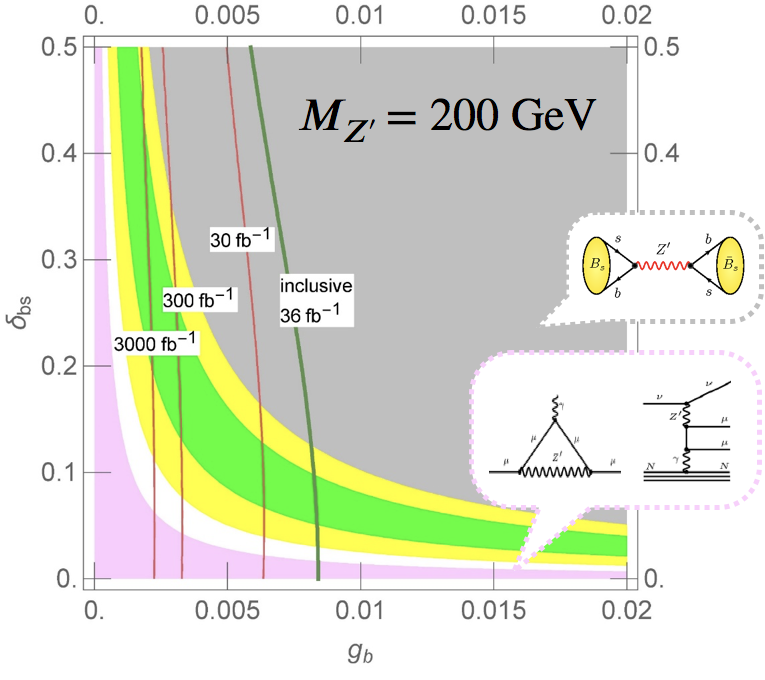
\includegraphics[width=8cm]{images/excluded_phase_space.png}
%    \caption{Reach of b-associated Z' search at the LHC compared to the inclusive search. %The top right grey area represents constraints from $B_s\rightarrow \bar{B}_s$ mixing, %the bottom left represents constraints from neutrino trident production/g-2, and the %green and yellow bands represent 1 and 2 standard deviation bands from the B %anomalies. We see that the b-associated Z' search (red) excludes more phase space than %the inclusive search (green).}
%    \label{fig:exc_pahse_space}
%\end{figure}


My dissertation focuses on the muonic decay of the Z'. Selecting for events containing dilepton ($e$ and $\mu$) pairs, low missing $E_T$, and at least one jet, we divide out sample into one and two jet, b-tagged and anti-btagged, and lepton permutation ($ee$, $e\mu$, $\mu\mu$) bins. We then employ three kinematic cuts to increase our significance: A $MET/M_{\ell\ell}$ (aka relative MET) filter takes advantage of the low transverse MET and high mass lepton pairs of the signal. Filtering on the difference between the hadronic transverse energy and letponic transverse energy (HT-LT) takes advantage of the fact that our associated b-jets tend to be "soft", or low energy. Finally, we permute the b-jets and leptons to create a best-guess top quark decay and compute it's mass (Top Mass Bound) to exclude top quarks from the final events. Cut values on these variables are optimized in monte-carlo simulation, and HT-LT and relative met cuts are optimized for variable mass points. Finally, an ABCD method is used to create a data driven background estimation, where we use electron vs muon and b-tagged vs anti-b-tagged regions to define our control and background regions. 

We are currently setting limits and finishing our analysis note. 

\section{Muon Alignment}

 Track based muon alignment is a critical alignment and calibration task at CMS. The alignment team is responsible for delivering up-to-date conditions of the positions of the muon detectors, ensuring the muon system is operating optimally, and developing further improvements to the muon alignment algorithm. I have contributed to all aspects of track based muon alignment since joining CMS in 2014, from delivering conditions under tight deadlines to ensuring proper data integrity, leading group and inter-group investigations, teaching and guiding new members of muon alignment, and developing new software for the track based muon alignment group based on modern programing practices and tools.
 
%Some examples of my contributions include working with other members of the team to upgrade muon alignment in the DTs from 3 to 6 degrees of freedom, upgrading our alignment validation code to function modularly and significantly more efficiently, leading multiple investigations into unexpected features in alignment, leading a study to measure overall systematic and statistical uncertainties, creating a simplified standalone monte-carlo simulation of the muon alignment algorithm for educational purposes and for directed investigations into hard to investigate systematics, branching the toy mc simulation of muon alignment into a project for a new student, helping guide development of GEM alignment, upgrading alignment software, representing the Muon Alignment group at AlcaDB/DPG meetings and much more. Our work in recent years is currently being summarized in a new Muon Alignment note. I will bring my leadership and innovation demonstrated by my work in muon alignment to future research. 
 
 
 \section{MonoTop}
 
 Exotic particle decays (e.g. certain non-thermal dark matter models) can result in single top production with right chirality at the LHC. Since standard model single top production results in mostly left-chiral tops, if we can measure the chirality of the top quark, we can gain a better handle on these processes. However, traditional top chirality measurements are designed to work with $t\bar{t}$ events and leverage correlations between the top quark decay products to measure chirality. e.g. the angle between the lepton angles of both pair-produced top quarks. At A\&M, we developed a simple single top observable to measure chirality in an event agnostic manner.
 
Our measurable relies on the relative energy difference a single top quark's daughter particles, allowing it to function independently of the top quark production mechanism. This not only makes it useful for our monotop search, but also as a general technique that could be applied to many top based analysis (e.g. precision standard model measurements). 

\section{Trajectory}


I am excited about the potential to work with the University of Minnesota's CMS group, work with computer and data scientists, contribute to the FAIR4HEP project, and continue to develop my physics, technical, data science, and leadership skills. I believe this postdoc would help me develop into a researcher that can contribute to a new generation of physics research and open doors in AI and data science for me. 



\bigskip

\begin{tabular}{@{}l@{}}
Sincerely, \\
  [.4em]
% \includegraphics[width=1.5in]{signature}\\ % my signature
  %[.2em]
  Ryan D. Mueller
\end{tabular}


\medskip

\printbibliography

\end{document}



%R. Allahverdi, M. Dalchenko, B. Dutta, A. Florez, Y. Gao, T. Kamon, N. Kolev, \textbf{R. Mueller}, and M. Segura. \href{https://link.springer.com/article/10.1007/JHEP12(2016)046}{``Distinguishing standard model extensions using monotop chirality at the LHC."} J. High Energ. Phys. (2016) 2016: 46. doi:10.1007/JHEP12(2016)046

